\begin{frame}{Neural Networks}
\begin{figure}
    \centering
    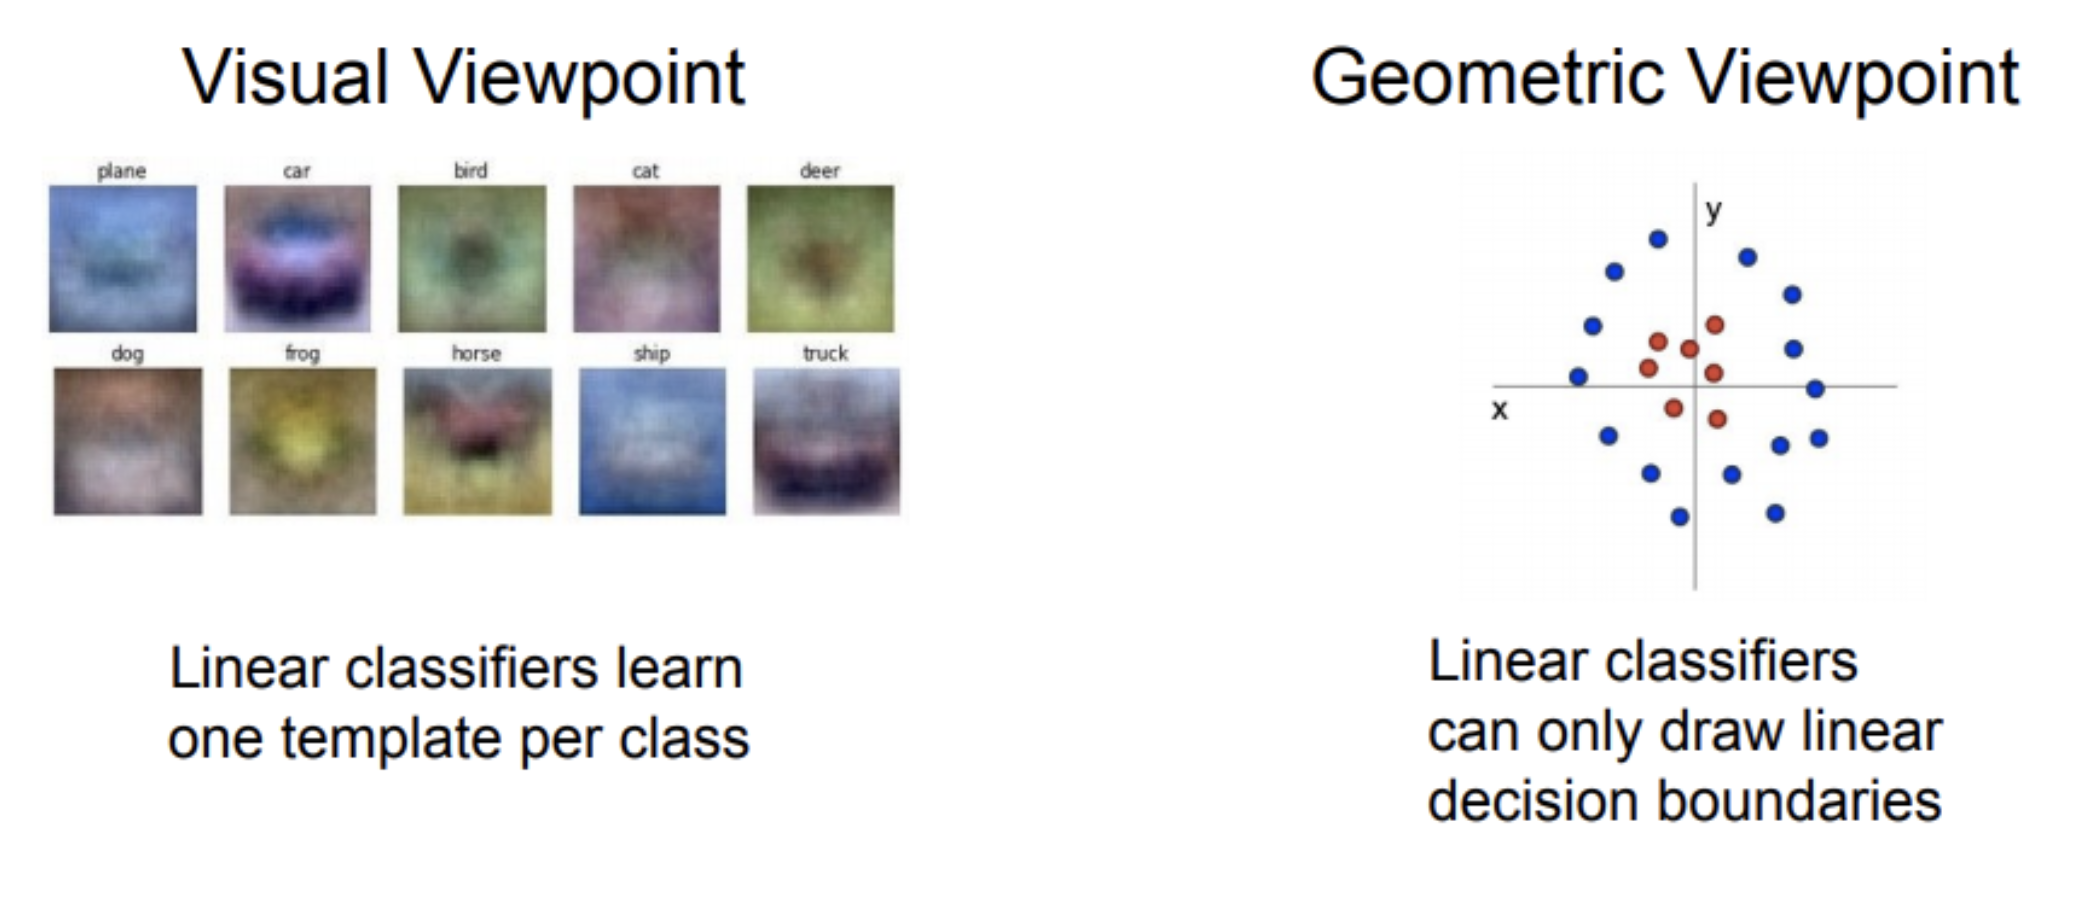
\includegraphics[width=\textwidth]{img/linearweak.png}
    \caption{Motivation: Linear models are fairly weak}
\end{figure}
\footnotetext{http://cs231n.stanford.edu/slides/2019/cs231n\_2019\_lecture02.pdf}
\end{frame}

\begin{frame}{Neural Networks}
\begin{itemize}
    \item We can model more complex functions by "stacking" more weights.
    \item Instead of
    $$\hat{y} = \sigma(\textbf{w} \cdot \textbf{x})$$
    We can now also do this:
    $$\hat{y} = \sigma(\textbf{w}_1 \cdot \sigma(\textbf{w}_2 \cdot \textbf{x}))$$
    $$\textbf{w}_1 \in \mathbf{R}^M, \textbf{w}_2 \in \textbf{R}^{M \times D}, \textbf{x} \in \textbf{R}^D$$
    Each row of the matrix $\textbf{w}_2$ is called a "neuron"
\end{itemize}
\end{frame}

\begin{frame}{Neural Networks}
\begin{figure}
    \centering
    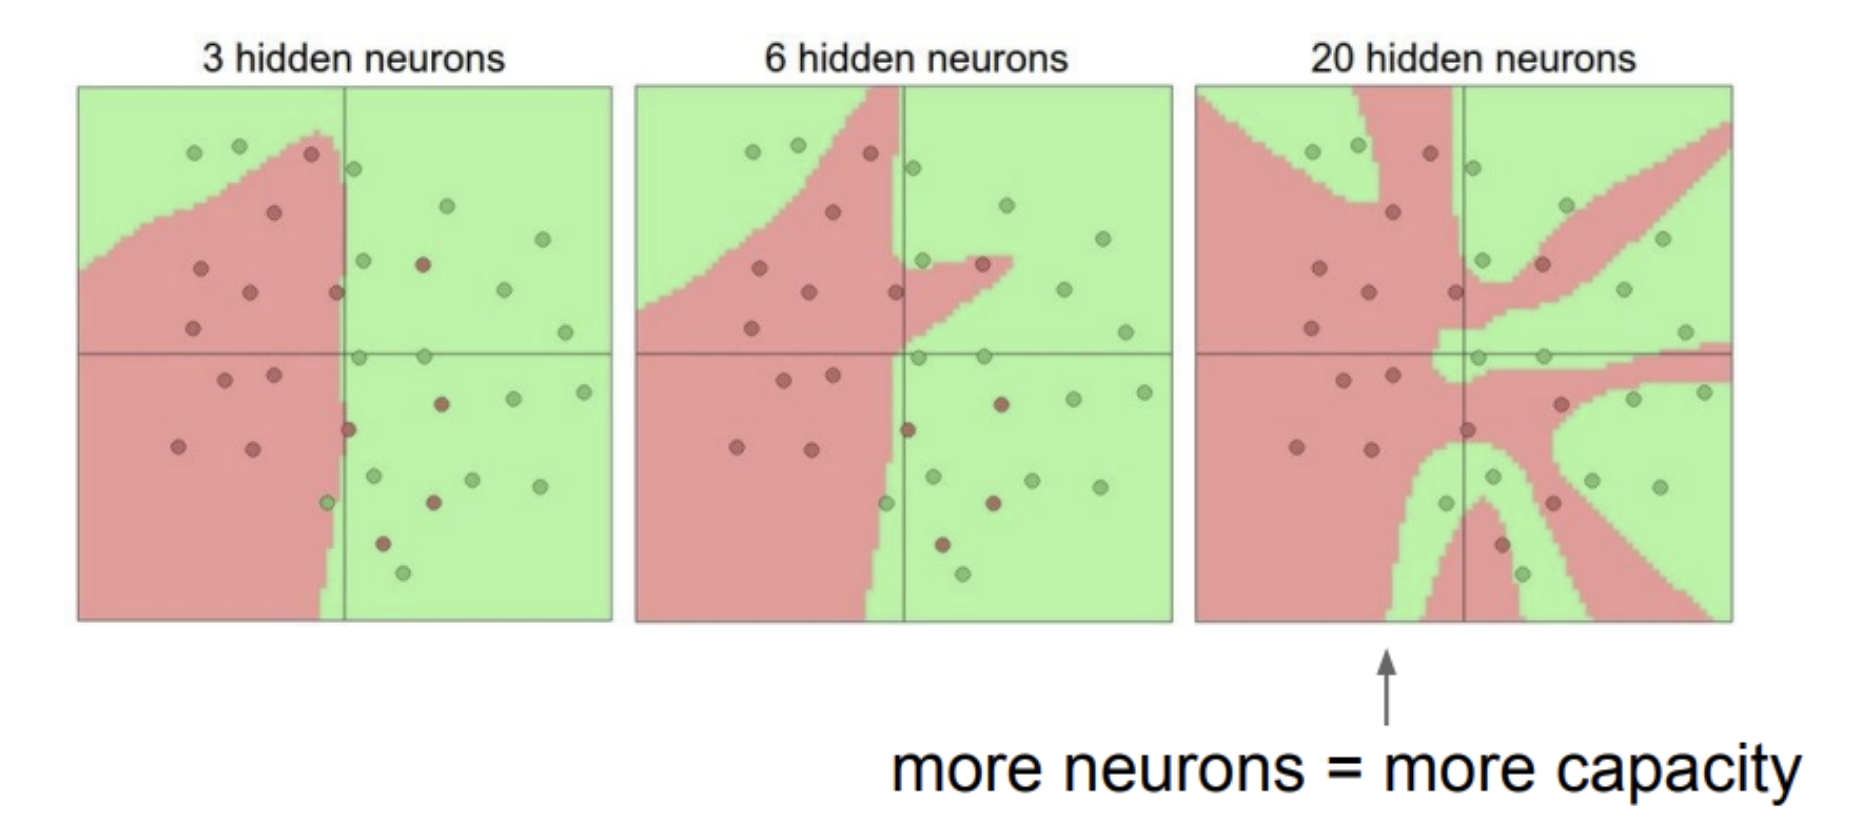
\includegraphics[width=0.8\textwidth]{img/moreneuronmorecap.png}
    \caption{The more neurons you have, the more \textbf{expressive} your model is.}
\end{figure}
\footnotetext{http://cs231n.github.io/neural-networks-1/}
\end{frame}

\begin{frame}{Neural Networks}
\begin{figure}
    \centering
    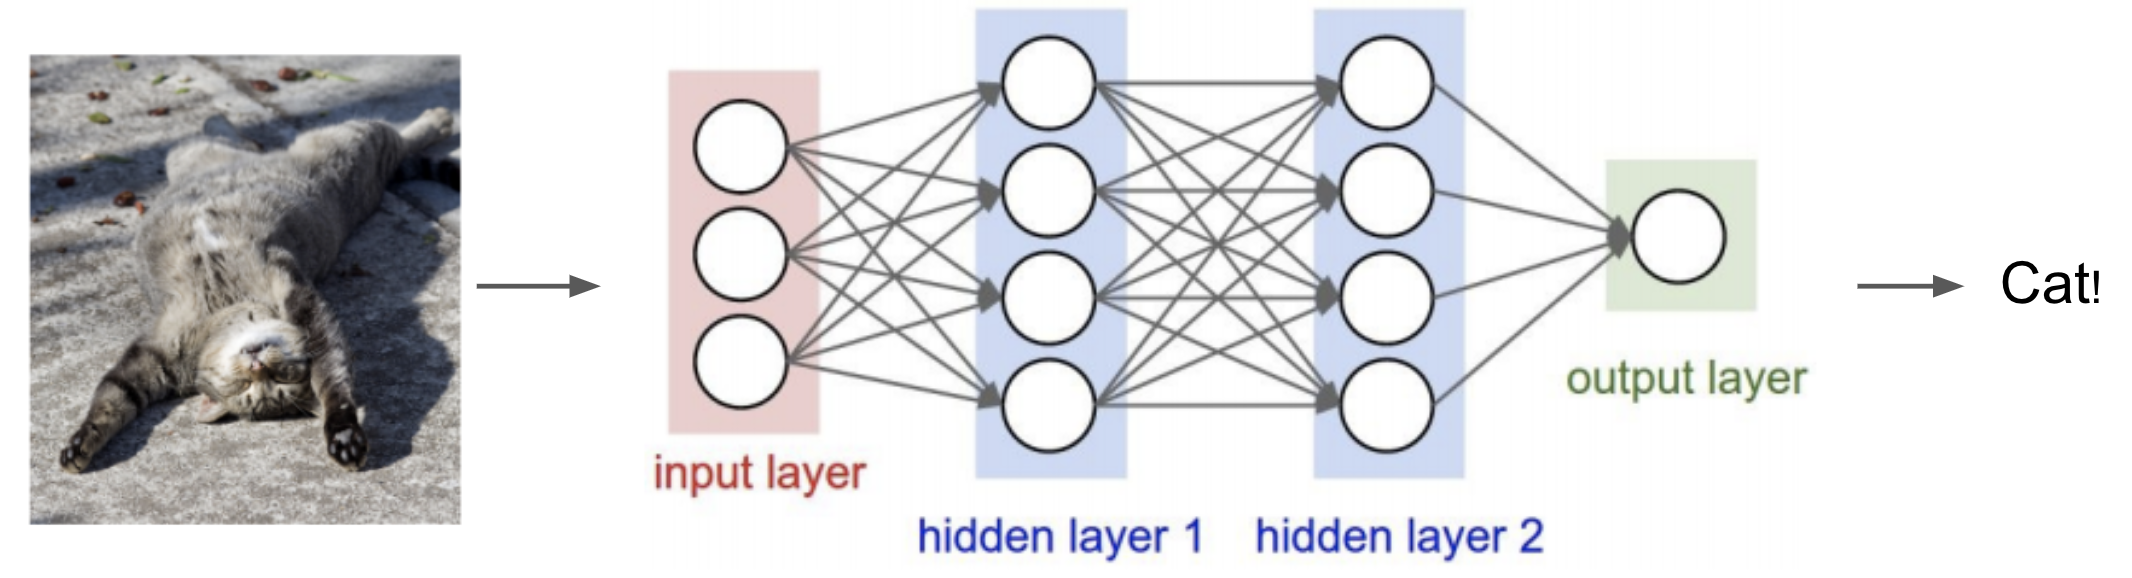
\includegraphics[width=\textwidth]{img/catNN.png}
    \caption{By stacking more and more layers and adding neurons, we can get models capable of representing all cats!}
\end{figure}
\end{frame}